\documentclass{standalone}
\usepackage{bm}
\usepackage{tikz}
\usetikzlibrary{angles,quotes}

\begin{document}
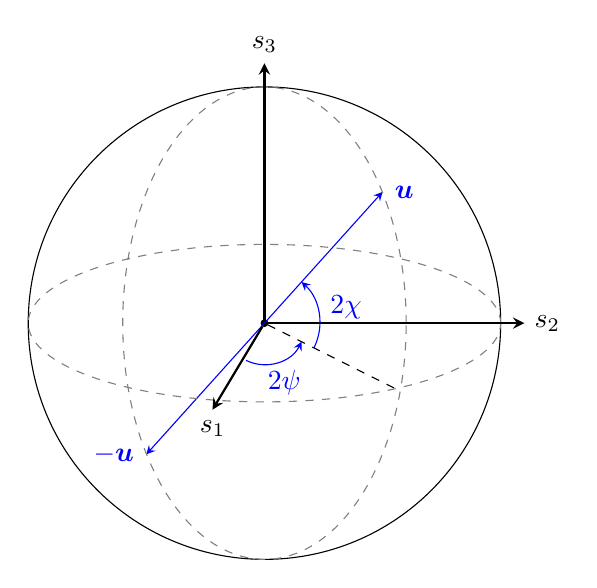
\begin{tikzpicture}

    % Radius
    \def\r{3}

    % Polarization vector
    \node[circle,fill,inner sep=1] at (0,0) {};
    
    \draw[->, >=stealth, blue] (0,0) node[inner sep=1] (orig) {} -- (\r/2,\r/1.8) node[inner sep=0.7,label=right:$\bm{u}$] (u) {};
    
    \draw[->, >=stealth, blue] (0,0) node[inner sep=1] (orig) {} -- (-\r/2,-\r/1.8) node[inner sep=0.7,label=left:$-\bm{u}$] (u2) {};
    
    %\draw[->, >=stealth, black] (0,0)  -- (0.7*\r/2,0.7*\r/1.8) node[inner sep=0.7,label=left:$V\bm{u}$] (a) {};
    
    \draw[dashed] (orig) -- (1.1*\r/2,-1.1*\r/4) node (phi) {};

    % Sphere
    \draw (orig) circle (\r);
    \draw[dashed, gray] (orig) ellipse (\r{} and \r/3);
    \draw[dashed, gray] (orig) ellipse ({0.60*\r} and \r{});
    
    
    % Axes
    \draw[->, >=stealth, thick] (orig) -- ++(-1.1*\r/5,-1.1*\r/3) node[below] (x1) {$s_1$};
    \draw[->, >=stealth, thick] (orig) -- ++(1.1*\r,0) node[right] (x2) {$s_2$};
    \draw[->, >=stealth, thick] (orig) -- ++(0,1.1*\r) node[above] (x3) {$s_3$};

    % Angles
    \pic [draw=blue,text=blue,->,"$2\psi$", angle radius=15, angle eccentricity=1.5, >=stealth] {angle = x1--orig--phi};
    \pic [draw=blue,text=blue,->,"$2\chi$", angle radius=20, angle eccentricity=1.5, >=stealth] {angle = phi--orig--u};

\end{tikzpicture}
\end{document}